%%%%%%%%%%%%%%%%%%%%%%%%%%%%%%%%%%%%%%%%%%%%%%%%%%%%%%%%%%%%%%%%%%
\documentclass[letterpaper, 10pt, conference]{ieeeconf}
\overrideIEEEmargins			% to meet printer requirements
\IEEEoverridecommandlockouts	% to override locked commands

%%%%%%%%%%%%%%%%%%%%%%%%%%%%%%%%%%%%%%%%%%%%%%%%%%%%%%%%%%%%%%%%%%
%REQUIRED PACKAGES%
\usepackage{multirow}
\usepackage{rotating}
\usepackage{float}
\usepackage{caption}
\usepackage{lipsum}
\usepackage{subcaption}
\usepackage{amsmath}
\usepackage{amssymb}
\usepackage{textcomp}
\usepackage{graphicx}
\usepackage{euscript}
\usepackage{ctable}
\graphicspath{{./Figures/}}
\usepackage[nonumberlist,acronym]{glossaries}
\usepackage[hidelinks]{hyperref}

%%%%%%%%%%%%%%%%%%%%%%%%%%%%%%%%%%%%%%%%%%%%%%%%%%%%%%%%%%%%%%%%%%

% correct hyphenation
\hyphenation{temp-orary}

% glossaries
\newacronym{ROS}{ROS}{Robot Operating System}

%%%%%%%%%%%%%%%%%%%%%%%%%%%%%%%%%%%%%%%%%%%%%%%%%%%%%%%%%%%%%%%%%%
\begin{document}

\title{Enhancing Autonomy of Mobile Robots with Behavioral Tree using ROS2}

\author{Lukas Evers$^{*,1}$, Umut Uzunoglu$^{1}$, and Ahmed Hussein$^{1}$ \textit{Senior Member, IEEE}%
    \thanks{$^{*}$ Corresponding author }%
    \thanks{$^{1}$ IAV GmbH, Berlin, Germany \newline
		{\tt\small lukas.evers@iav.de, umut.uzunoglu@iav.de, ahmed.hussein@ieee.org}}%
}

\maketitle
\pagestyle{empty}

%%%%%%%%%%%%%%%%%%%%%%%%%%%%%%%%%%%%%%%%%%%%%%%%%%%%%%%%%%%%%%%%%%

\begin{abstract}

This paper proposes a state of the art review and a behavioral planning approach to improve the autonomy of mobile robots using the Robot Operating System (ROS2). The study aims to address the issue of human intervention that is often required during the operation of autonomous mobile robots and improve the efficiency and performance of the robots. The system includes a monitoring system, sensor data storage, and behavior tree design and implementation. The effectiveness of the approach was evaluated using the Gazebo simulator, with the behavior tree handling various scenarios such as sensor failures, collisions, unreachable goals, and low battery state. The simulation results showed a significant improvement in the robot's autonomy and resilience to failures, providing evidence for the feasibility of the proposed approach. To further validate the results, additional experiments are being performed in real-world settings.

\end{abstract}

%%%%%%%%%%%%%%%%%%%%%%%%%%%%%%%%%%%%%%%%%%%%%%%%%%%%%%%%%%%%%%%%%%

\section{Introduction}
\label{sec:Introduction}

Mobile robots are increasingly being used in a variety of fields, including warehouse logistics, last-mile delivery, and agriculture. Despite being marketed as autonomous, they often require human supervision to operate correctly and are limited in their autonomy to specific environments. The Robot Operating System (ROS) is a popular platform for building and programming robots, but the standard robot still requires human intervention to ensure proper functioning and safety in uncertain environments.

This paper focuses on how behavior planning can increase the robustness and autonomy of robots running ROS2. Behavior planning allows the robot to react to failures and problems and decide on alternative courses of action to mitigate risks and achieve its goals. The paper will explore the possibility of improving current systems by adding a dedicated behavior planning component and provide an implementation of exemplary behaviors and a system architecture for incorporating behavior planning in other robots.

The study aims to demonstrate that the implementation of behavior planning can increase the robot's robustness and decrease the need for human intervention in various scenarios. The paper will present the results obtained from selected scenarios, where failures and problems will be artificially induced to test the robot's ability to behave autonomously. The paper will summarize the results and discuss the acceptance criteria for the requirements. The conclusion will provide an outlook for future work and recommendations.

%%%%%%%%%%%%%%%%%%%%%%%%%%%%%%%%%%%%%%%%%%%%%%%%%%%%%%%%%%%%%%%%%%

\section{State of the Art}
\label{sec:StateOfTheArt}

\subsection{Autonomous Driving Navigation Architectures}

Autonomous driving software architectures follow the "\textit{Sense - Think - Act}" paradigm \cite{murphy2000}, as shown in Figure \ref{fig:autonomous_driving_architecture}. Most architectures implement a hierarchical structure in which sensory inputs are processed to create an environmental representation, leading to a path from the current position to the destination computed by global planning. This is followed by behavioral planning, which ensures that the vehicle obeys traffic rules, and local planning, which translates motion commands while taking into account system constraints. An additional system monitoring layer monitors the execution of other components and triggers actions in case of failures \cite{zimmermann2020adaptive}. Vehicles can achieve (Society of Automotive Engineers) SAE levels of autonomy up to levels four and five \cite{bacha2008odin}. Expanding the behavior planning module can lead to higher levels of autonomy \cite{reke2020}.

\begin{figure}[ht]
	\centering
	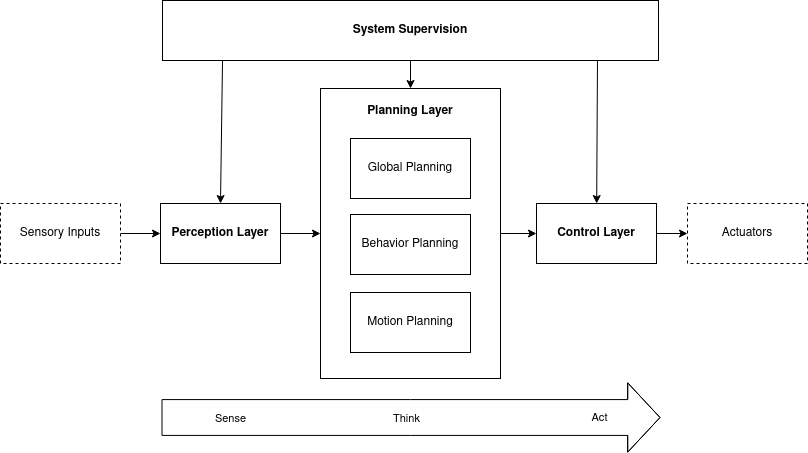
\includegraphics[width=0.9\linewidth]{Figures/autonomous_driving_architecture.png}
	\caption{Common Autonomous Driving Architecture \cite{brooks1986,velasco2020}}
	\label{fig:autonomous_driving_architecture}
\end{figure}

\subsection{Behavior Types}

The behavior planning module is responsible for choosing the best behavior to execute in a specific environment to ensure the best performance for a given task. A behavior planning approach provides the robot with acceptable behaviors for every possible scenario the robot is operating in.

\subsubsection{Reactive Approach}

The first type of behaviors implemented in behavior-based robots were reactive behaviors. This maps sensory input directly to motor commands, similar to reflexes in humans. Reactive behaviors are fast due to their low computational load, and are suitable in scenarios where real-time safety is a concern. However, a system with a solely reactive behavior planning approach will not meet requirements for higher levels of autonomy. Reactive behaviors can still be valuable in improving vehicle safety and reliability \cite{desilva2008}.

\subsubsection{Deliberative Approach}

Deliberative behaviors are defined as behaviors that involve planning and decision-making. Unlike reactive behaviors, deliberative behaviors follow the "Sense, Think, Act" paradigm and can decide the best course of action before acting \cite{murphy2000}. A behavior planner with a deliberative approach can make decisions based on current and previously processed data, and can predict environmental changes. Deliberative behaviors improve autonomy and mimic human skills, reducing the need for a human operator.

\subsubsection{Hybrid Approach}

A hybrid model combining reactive and deliberative behaviors can create reliable and intelligent systems. The hybrid approach combines the quick reaction times of reactive behaviors with the decision-making ability of deliberative behaviors, leading to more robust robots and higher levels of autonomy. The higher-level deliberative planners can override reactive planners, allowing the system to be more flexible in uncertain environments while still maintaining fast reaction times \cite{arkin1998}.

\subsection{Behavior Planning Approaches}

Robots that use a hierarchical behavior planning approach need a system to determine which behaviors to execute. Different approaches for behavior planning use states to determine which strategies and behaviors are utilized. This article presents and compares Finite State Machines (FSMs), Behavior Trees (BTs), and Partially Observable Markov Decision Processes (POMDPs).

\subsubsection{Finite State Machines}

FSMs are a popular choice for behavior planning in robotics. The fundamental idea behind FSMs is to describe behavior in terms of states that trigger actions. FSMs are defined by a set of states, a starting state, state transitions, final states, and an input alphabet. At any given time, a specific state machine is selected and its actions are executed. The benefits of FSMs include their speed and ease of implementation, especially when using libraries, which can make the development process much simpler and faster. However, as the complexity of the problem increases, so does the effort required to implement the FSM. Despite these limitations, FSMs are still a widely used approach in robotics due to their simplicity and effectiveness in controlling motors \cite{wagner2006}.

\subsubsection{Behavior Trees}

BTs are a popular approach for modeling AI for non-player characters in computer games. Unlike FSMs, BTs have a hierarchical structure, with nodes that represent actions or sequences of actions. The tree consists of a root node, child nodes, parent nodes, and leaf nodes (execution or action nodes). The behavior tree is executed by ticking the root node, which will then be recursively ticked down the tree until the execution of an action node is triggered. Control nodes, such as "Sequence," "Fallback," and "Condition," determine the order and conditions of execution for the action nodes. BTs provide a flexible and intuitive way to represent complex AI behaviors, and are widely used in the game development industry \cite{iovino2022}.

\subsubsection{Partially Observable Markov Decision Processes}

POMDPs are a more sophisticated approach for decision-making in uncertain environments. The basic idea behind POMDPs is to model decision-making as a process of choosing actions based on the probability distribution of the system's state. A POMDP consists of a set of states, actions, observations, rewards, and a transition model. POMDPs use belief states, which represent the probability distribution of the system's state, to make decisions. The solution to a POMDP is a policy, which is a mapping of belief states to actions. POMDPs are more complex than FSMs and BTs, but provide a more robust and flexible way to handle uncertainty in robotic decision-making \cite{feyzabadi2014riskaware}.

In conclusion, the behavior planning module of an autonomous driving system plays a crucial role in determining the best behavior to execute in a given environment. The behavior planning approach can range from reactive to deliberative to a hybrid of both. FSMs and BTs are two popular approaches for behavior planning in robotics, while POMDPs are a more sophisticated approach for decision-making in uncertain environments. FSMs are fast and easy to implement, while BTs provide a flexible and intuitive representation of complex AI behaviors. POMDPs are more complex but provide a robust and flexible way to handle uncertainty. The proposed approach for this study will use a BT approach for the behavior planning module, offering a hierarchical structure for modeling AI and a flexible representation of complex behaviors.

%%%%%%%%%%%%%%%%%%%%%%%%%%%%%%%%%%%%%%%%%%%%%%%%%%%%%%%%%%%%%%%%%%

\section{Proposed Approach}
\label{sec:ProposedApproach}

In this work, the Robot Operating System 2.0 (ROS2) \cite{ros2022} framework was selected as the platform to test the hypothesis. ROS2 is a newer version of the open-source middleware, Robot Operating System (ROS) \cite{quigley2009}, that has received updates to its architecture and design for improved real-time safety, certification, and security for industrial applications. ROS2's Nav2 package, which is used for navigation and localization, has some limitations. For example, it may not handle events such as slipping wheels or orientation changes by external influences appropriately. This can lead to erratic movement of the robot, as well as incorrect planning commands. In severe cases, the robot may continue to drive despite incorrect interpretation of its surroundings, which is highly unsafe and requires manual intervention. Therefore, to achieve higher levels of autonomy, it is necessary to define requirements that address these limitations and elevate the level of safety and reliability.

\subsection{Requirements}

The limitations of the standard ROS and Navigation2 setup for mobile robots were identified and used to derive software requirements for improving the robot's behavior. The non-functional requirements and their descriptions are listed in Table \ref{tab:fn_req}. The functional requirements and their acceptance criteria are also listed in the same table, with prioritization based on the severity of consequences for the system. The first six functional requirements prioritize safety and robustness, while functional requirements seven to nine focus on increasing robot autonomy with lower risk potential.

\begin{table*}[ht]
	\centering
	\caption{Non-Functional and Functional Requirements}
	\label{tab:fn_req}
	\renewcommand{\arraystretch}{1.25}
		\begin{tabular}{|m{0.06\textwidth}|m{0.15\textwidth}|m{0.05\textwidth}|m{0.64\textwidth}|} 
			\hline
			\textbf{Nr.} & \textbf{Name} & \textbf{Priority} & \textbf{Description/Acceptance criteria} \\ 
			\hline
			non$\_$freq1 & Single Point of Failure & High & The system does not have a single point of failure. If parts of the system fail, the system maintains some level of functionality. \\ 
			\hline
			non$\_$freq2 & Performance & High & The control loop of the system guarantees fast reactions. The average frequency at which the system operates is higher than 100Hz (10ms). \\ 
			\hline
			non$\_$freq3 & Determinism & High & The outcome for a given set of inputs must be deterministic, which means that the behavior will always be executed in a similar way. \\
			\hline
			non$\_$freq4 & Deliberate & High & The robot is able to perform deliberative behaviors, which means that the newly implemented behaviors go beyond the reaction to the sensor input and have a planning aspect. \\
			\hline
			fn$\_$req1 & Sensor Failure & High & The system detects sensor failure. Ensure that the system can restart sensors and decrease the speed during the time the sensor delivers limited information. \\ 
			\hline
			fn$\_$req2 & Emergency Detection & High & The system detects emergency. Ensure that the system can detect when the continuation on the calculated path is no longer safe (sensor failures, blockage). \\
			\hline
			fn$\_$req3 & Emergency Stop & High & The system can initiate emergency stops. Ensure that the system can override all commands and stop in case an emergency is detected. \\
			\hline 	
			fn$\_$req4 & Override Navigation2 & High & The system can override navigation2. Ensure that the system's commands can always override the commands coming from navigation2. \\
			\hline
			fn$\_$req5 & Maintain operability & High & The robot executes commands as long as it is safe. Ensure that the robot keeps driving if it is safe even when system functions are not working correctly. \\
			\hline
			fn$\_$req6 & Recovery & High & The system can recover from crashes. Ensure that the system can successfully reach goals despite previous crashes.\\ 
			\hline 
			fn$\_$req7 & Control Path Planning & Medium & The system controls and rates the quality of the planned paths. \\
			\hline	
			fn$\_$req8 & Reset Goals & Medium & The system can reset and override goals set by the user so that the goal is reachable by planners. \\
			\hline
			fn$\_$req9 & Robot Range & Medium & Ensure that the robot will not run out of battery during navigation to a goal. \\	
			\hline
		\end{tabular}
\end{table*}

\subsection{System Solution}

This work focuses on extending the capabilities of a mobile robot system by adding an autonomous layer to the existing navigation setup. The requirements for improving the robot's behavior were derived from the limitations of the current setup and are prioritized based on their severity. The autonomy layer is designed to increase the robustness and autonomy of the whole system and includes three main components: a system supervisor, a data storage system, and a behavior planner. The system supervisor monitors the health of all components, including sensors and navigation, and provides constant execution monitoring. The data storage system stores relevant system information and data, allowing for more deliberative behaviors. The behavior planner processes information from the execution checker, the navigation system, and sensor data to make decisions on how to increase autonomy. Finally, a decision gate is needed to intelligently switch between speed commands from the navigation system and the autonomy layer. A block diagram of the proposed system is shown in Figure \ref{fig:block_diagram}.

\begin{figure}[ht]
	\centering 
	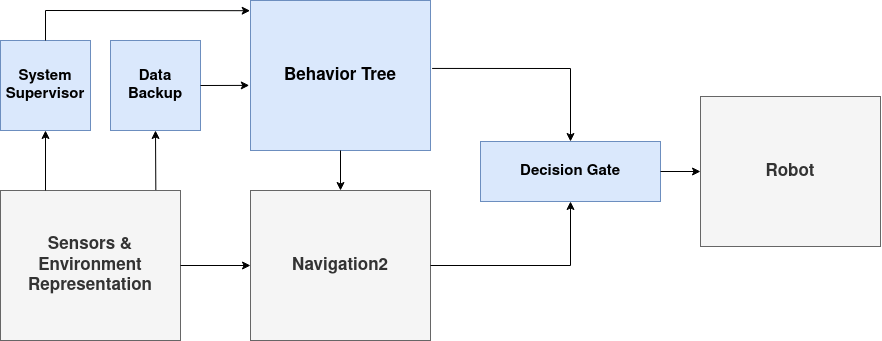
\includegraphics[width=0.9\linewidth]{Figures/block_diagram.png}
	\caption{Proposed System Block Diagram: The additional components, discussed in this work, are colored blue while the existing components are colored gray}
	\label{fig:block_diagram}
\end{figure}

\subsection{Software and Simulation}

The paper compares and assesses behavior planning approaches, eventually choosing the behavior tree method for its increased flexibility and determinism. The Nav2 stack implements behavior trees using the Behaviortree.CPP (BT.CPP) library, which provides a way to create, execute, monitor, and edit behavior trees and allows communication between nodes. The behavior trees can be created using the Groot software, which is a graphical user interface for creating, editing, and debugging behavior trees. The behavior trees are developed and tested using the Gazebo simulator and the Turtlebot3 model. The simulator allows for easier testing and offers control over the simulation time. The software versions used are with the choice of using ROS2 Foxy and C++ for development.

\subsection{System Architecture}

The system architecture in Figure \ref{fig:component_diagram} shows the integration of the autonomy layer into current architecture, with existing components in gray and new components (Data Backup, Decision Gate, Behavior Tree, and System Supervisor) in blue. The System Supervisor is explained in the BT section, as it's part of the behavior tree's functionality.

\begin{figure}[ht]
	\centering
	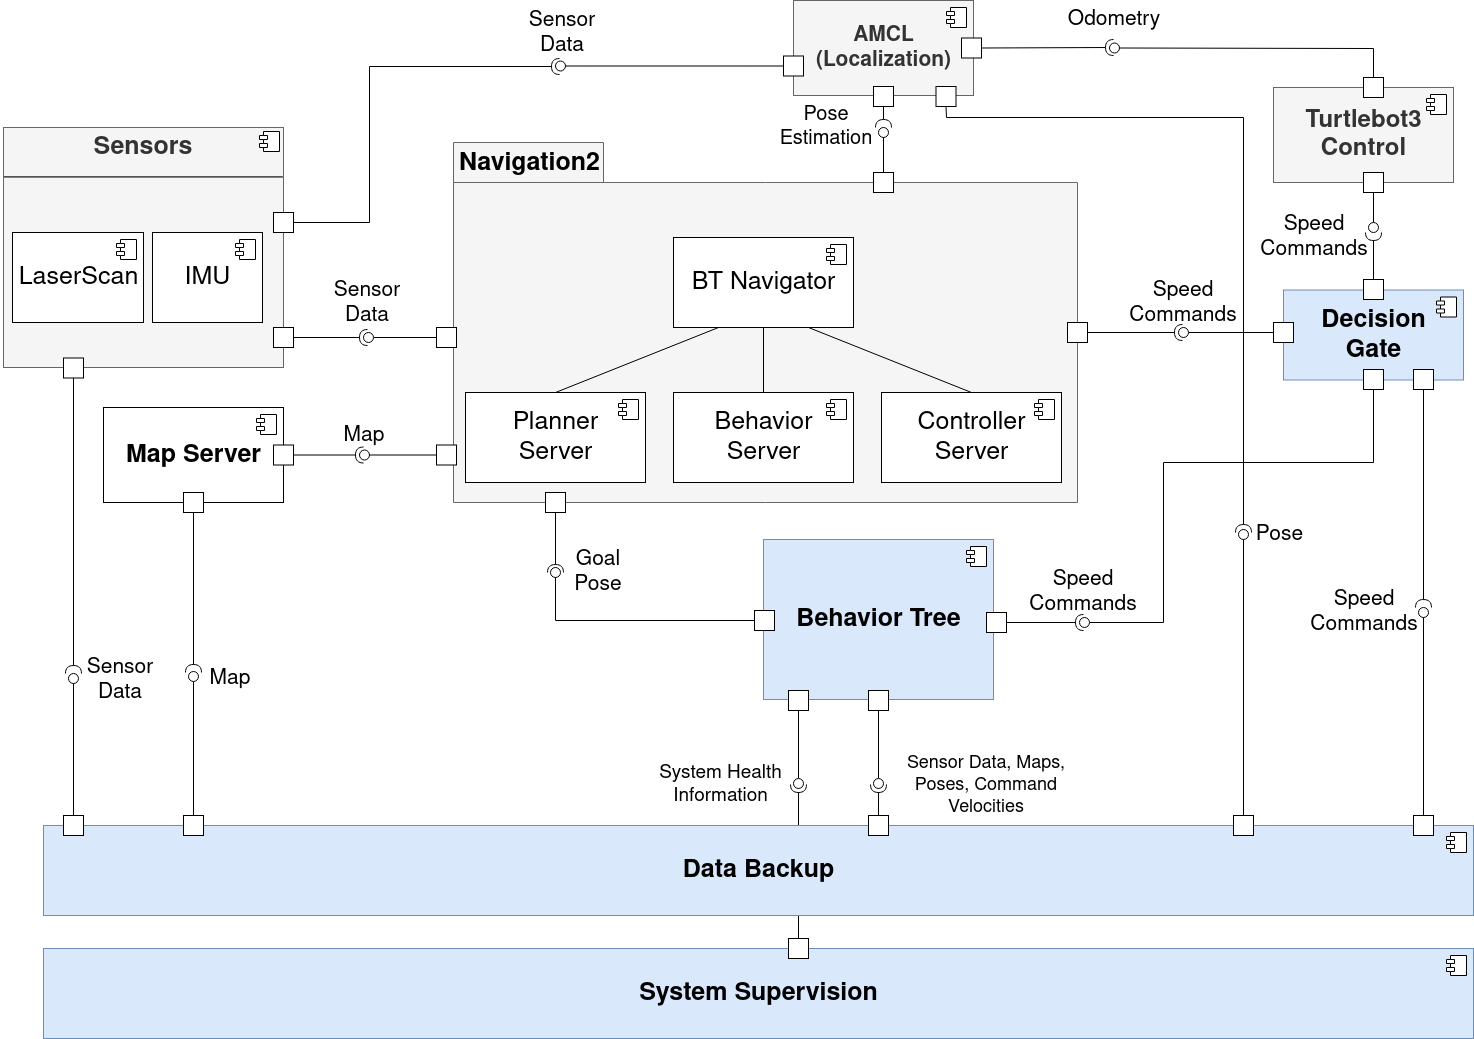
\includegraphics[width=0.9\linewidth]{Figures/component_diagram_bt.png}
	\caption{Component Diagram of System Architecture}
	\label{fig:component_diagram}
\end{figure}

The data backup component gathers data from system components and provides it to the behavior tree for past data points. It subscribes to sensor data and saves the messages in a queue data structure. The array size is limited to decrease network load and computational requirements. The behavior tree accesses the saved data through a service call to one of the component's services. The data backup component operates in a separate ROS node to avoid blocking the execution of the autonomy system.

The decision gate component modifies or blocks velocity commands from Nav2. It receives messages from Nav2 and the behavior tree, and prioritizes messages from the behavior tree. The component is an added safety measure in case Nav2 is not responsive to a cancellation command.

The system supervisor component uses a Watchdog design pattern to monitor the system and take corrective measures when problems are detected. The component operates partly outside the behavior tree's thread to avoid blocking its execution. The component receives messages from nodes and informs the behavior tree of problems with a node through a provided service. The behavior tree uses service calls to check component health in Condition Nodes. If a node fails, the robot slows down and tries to restart the sensor. If the restart fails twice, the robot stops. The timeout for declaring a node failed is set to one second.

\subsection{Behavior Tree Structure}

The top-level behavior control fallback nodes of a simplified behavior tree are shown in Figure \ref{fig:top_level_bt}. The tree receives the tick signal from a sequence root node. The root node functions to increase the system's robustness by ensuring all fundamental components are functioning properly before executing higher-level behaviors. Details for each behavior will follow.

\begin{figure*}[ht]
	\centering
	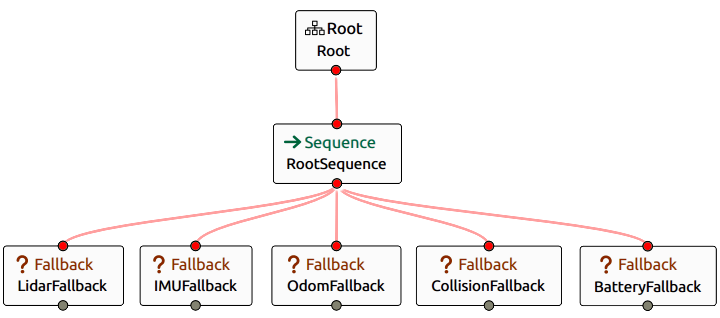
\includegraphics[width=0.9\linewidth]{Figures/top_level_bt.png}
	\caption{Top Level Behavior Tree Structure}
	\label{fig:top_level_bt}
\end{figure*}

The robot's collision behavior is meant to handle collisions and react to them. Collisions occur due to inadequate sensor coverage or a lack of detection capabilities. The collision behavior involves detecting a collision, getting out of the collision state, updating the map, and resetting all costmaps to generate a new path to the goal. The collision checker uses a simulated sensor and is integrated into the system supervisor. The behavior tree (BT) requests the most recent command velocities and modifies them to reverse out of the collision. The map needs to be updated with a new obstacle at the collision point and republished. The estimated collision point is simplified to be directly in front of the robot, and a square with 100\% occupancy is added to the map. The original goal is then republished to replan the global path.

The battery behavior monitors the robot's battery and decides if the robot should navigate to a new goal location. The decision is based on the current battery charge and the estimated energy consumption to reach the new goal. The energy expenditure was predicted using a linear function and considering the idle consumption and energy to drive the motors. A safety factor was added to the energy estimation function to consider scenarios where the robot may need to stop navigation.. A battery package was created for simulation purposes and updates the battery charge every second. The battery package subscribes to the command velocity topic and decreases the battery charge for every message received. The consumption rates are not close to reality but were chosen for rapid testing.

The path planning behavior involves generating a safe path for the robot to navigate from its current location to a goal location. The path is generated based on the robot's current location, goal location, and the environment. The path planning behavior makes use of the map data and costmaps to generate a path that avoids obstacles. The costmap is updated with the new obstacle information to ensure the path is safe. The global and local planners generate a path, and the velocity commands are sent to the robot. The robot's velocity is monitored, and if it deviates from the planned path, the path is replanned to ensure the robot stays on course.

\subsection{ROSBot Adaption}
   
The ROSBot 2.0 by Husarion has been selected as the test platform for real world scenarios. It is a four-wheeled robot equipped with a suite of sensors, including LiDAR, IMU, wheel encoders and range sensors. To advance the ROSBot to a higher level of autonomy the proposed system architecture has been implemented. The battery charge module and the collision detection module were required to be adapated from the simulation to function on the real robot. The collision detection module is based on the IMU data instead of a simulated bumper sensor.

The battery module estimates the remaining charge by taking the battery voltage, the power consumption of every component and the movement of the robot into account thus assuring that the robot has enough charge left to navigate to a given goal. Following function is used to determine the current state of charge of the battery: \[Batt_{SoC}(t) = Batt_{SoC}(t-1)-\frac{\frac{P_{components}}{V_{measured}}}{Batt_{capacity}}* t_{timestep} *100\] where $Batt_{SoC}$ is the charge in percentage, $t$ is the time of calculation in hours, $t_{timestep}$ the time step in seconds and $P_{components}$ the combined power consumption of every component connected to the robot in Watt. $P_{components}$ changes depending on the speed of the robot. The calculation assumes a fully charged battery.

\section{Results and Discussion}
\label{sec:ResultsAndDiscussion}

\subsection{Setup}

The efficacy of the behavior tree component in the robot was evaluated through scenario testing in a simulated apartment environment (as shown in Figure \ref{fig:house_gazebo}) and a simulated world with small round obstacles in an enclosed space (as shown in Figure \ref{fig:world_gazebo}). These scenarios were designed to trigger behavior responses from the component and to assess its ability to meet the functional requirements specified earlier. The environments were pre-mapped using the ROS2 "SLAM Toolbox" package and provided by the Nav2 map server. The robot location and navigation goals were defined in a separate ROS node, which programmatically positioned the robot within the environment and set its goals. This approach allowed the same scenario to be run with and without behavior planning. To test the behavior of the sensor failure fallbacks, the relevant sensor driver was shut down to emulate sensor failure.

\begin{figure}[ht]
	\centering
	\begin{subfigure}[b]{0.49\linewidth}
		\centering
		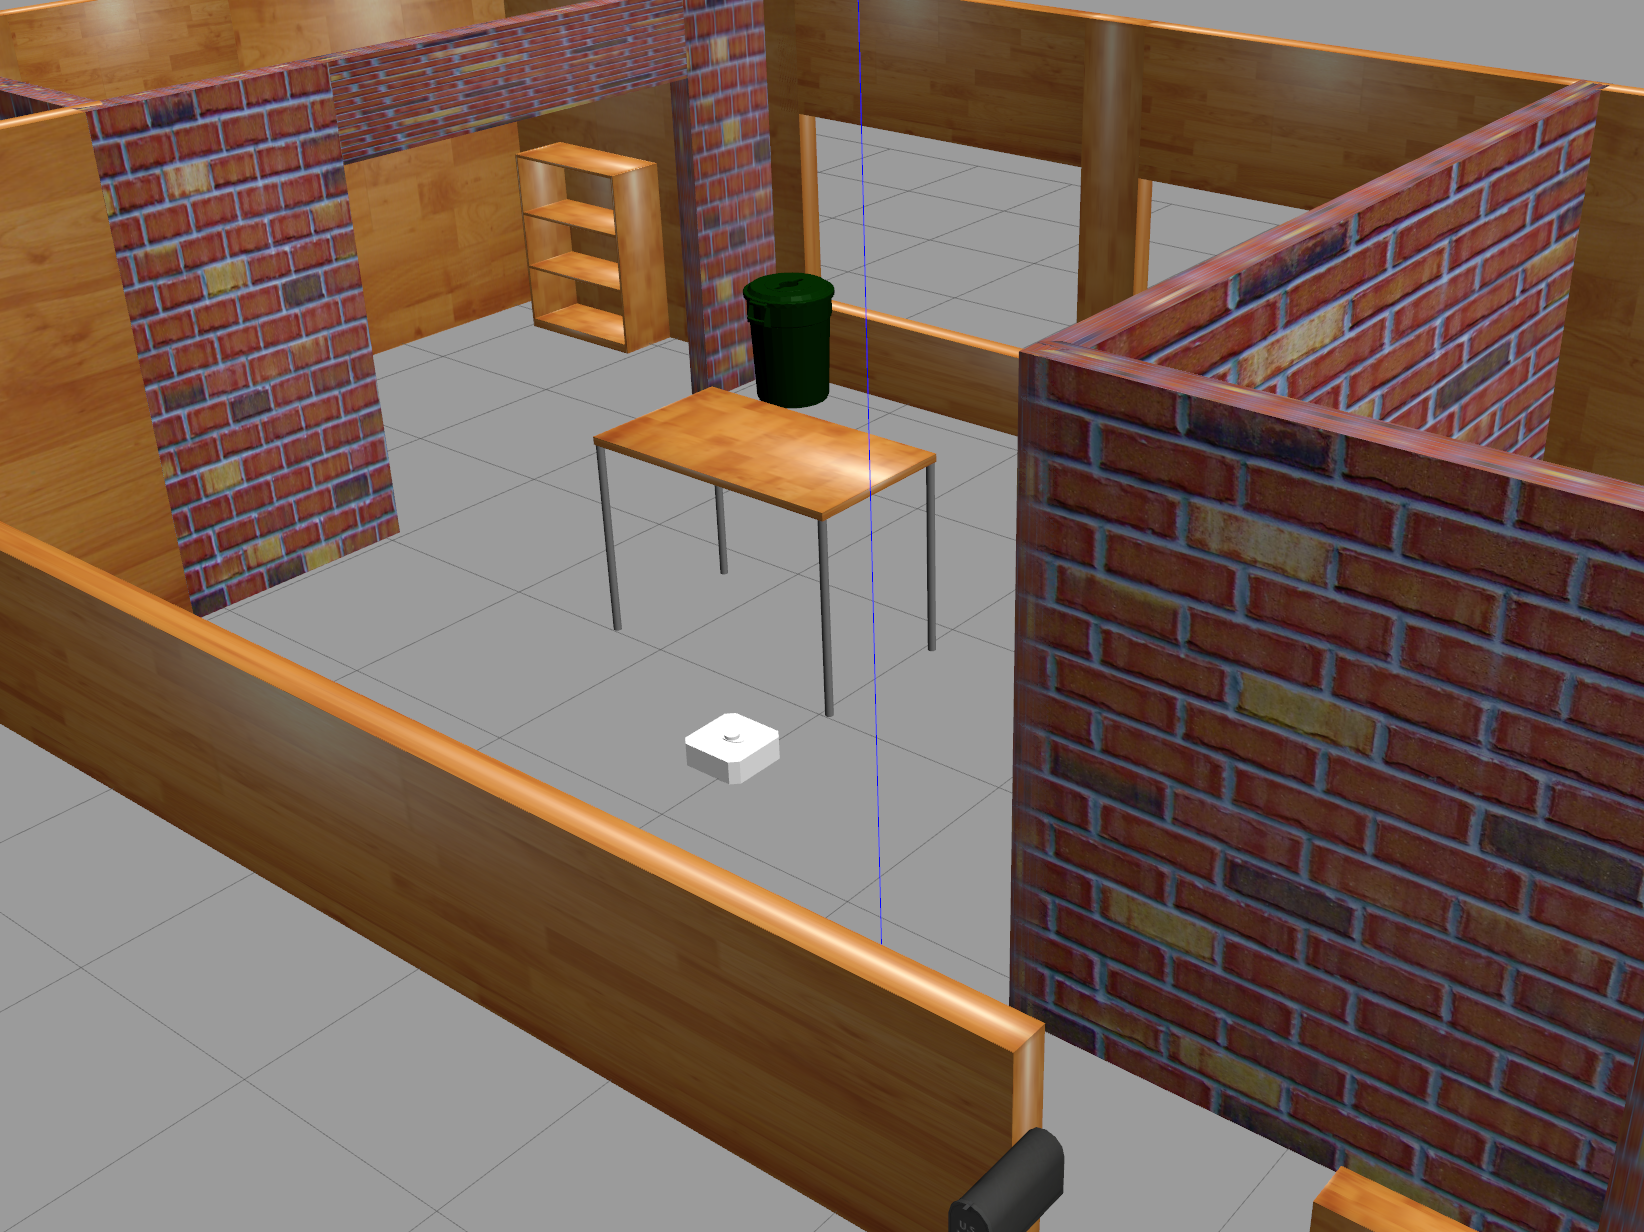
\includegraphics[width=\linewidth]{Figures/house_env.png}
		\caption{Apartment Environment}
		\label{fig:house_gazebo}
	\end{subfigure}
	\hfill
	\begin{subfigure}[b]{0.49\linewidth}
		\centering
		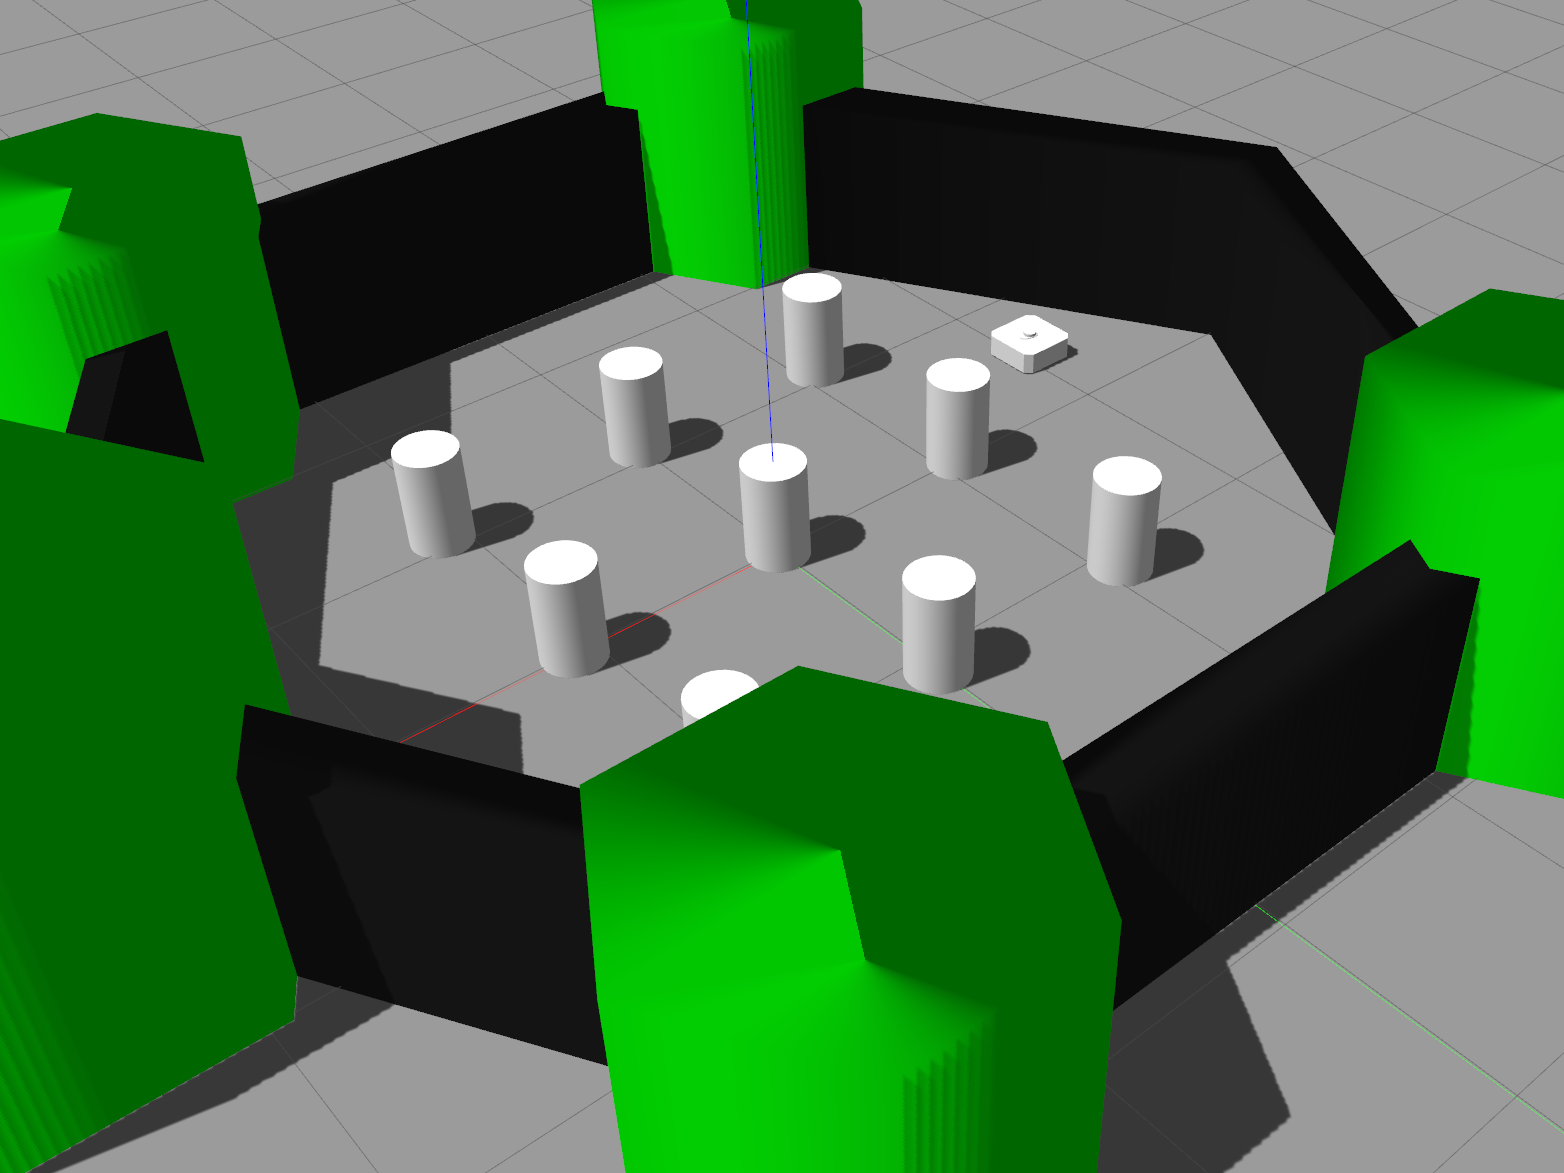
\includegraphics[width=\linewidth]{Figures/world_env.png}
		\caption{Enclosed Environment}
		\label{fig:world_gazebo}
	\end{subfigure}
	\caption{Gazebo World Environment}
	\label{fig:three graphs}
\end{figure}

\subsection{Scenarios}

The scenarios, derived from functional requirements, test multiple requirements as listed in tables \ref{tab:behavior_scenarios} and \ref{tab:sensor_scenarios}. To be counted as a success, all acceptance criteria for a scenario must be met. The scenarios are conducted by shutting down sensor drivers, publishing navigation goals, and simulating obstacles and battery conditions. Examples include: NoPathFound$_1$ tests recovery from inability to plan, NoPathFound$_2$ tests alternative goal navigation, Collision$_1$ tests maneuvering out of collisions, Collision$_2$ tests recovering from crashes, and Battery$_1$ tests low battery navigation.

\begin{table}[ht]
	\centering
	\caption{Behavior Scenarios}
	\label{tab:behavior_scenarios}
	\renewcommand{\arraystretch}{1.25}
	\resizebox{0.95\linewidth}{!}{%
		\begin{tabular}{| m{0.11\linewidth} | m{0.19\linewidth}| m{0.4\linewidth} | m{0.3\linewidth}|} 
			\hline
			\textbf{Name} & \textbf{Requirements} & \textbf{Description} & \textbf{Success Criteria}\\ 
			\hline	
			NoPath Found$\_$1 & fn$\_$req7 & Path to goal can not be calculated, robot is standing still & 
			Reset system, calculate path to goal, reach goal \\
			\hline
			NoPath Found$\_$2 & fn$\_$req7, fn$\_$req8 & Goal is unreachable, robot is standing still & Alternative goals, close to the original are tested to be reachable \\
			\hline
			Collision$\_$1 & fn$\_$req2, fn$\_$req4, fn$\_$req6 & Robot is standing still and a collision with the robot is caused & Robot can get out of collision state, navigation to goals still working \\
			\hline
			Collision$\_$2 & fn$\_$req2, fn$\_$req4, fn$\_$req6 & The robot is driving and collides with an undetected obstacle (0.25m/s) & 
			Robot can get out of collision state, navigation to goals still working, undetected obstacle gets added to map \\
			\hline
			Battery$\_$1 & fn$\_$req9 & The robot battery runs low & The robot will not drive to a goal that is outside of its reachable range \\
			\hline	
		\end{tabular}
	}
\end{table}	

\begin{table}[ht]
	\centering
	\caption{Sensor Scenarios}
	\label{tab:sensor_scenarios}
	\renewcommand{\arraystretch}{1.25}
	\resizebox{0.95\linewidth}{!}{%
		\begin{tabular}{| m{0.1\linewidth}| m{0.1\linewidth} | m{0.2\linewidth}| m{0.3\linewidth} | m{0.3\textwidth}|} 
			\hline
			\textbf{Sensor Tested} & \textbf{Name} & \textbf{Requirements }& \textbf{Description} & \textbf{Success Criteria}\\ 
			\hline
			& Lidar$\_$1 & fn$\_$req1, fn$\_$req2, fn$\_$req3, fn$\_$req4, fn$\_$req5 & Robot is standing still, Lidar node crashes & Reset the system\\ 
			\cline{2-5}
			Lidar &Lidar$\_$2 & fn$\_$req1, fn$\_$req2, fn$\_$req3, fn$\_$req4, fn$\_$req5 & Navigating with 0.25 m/s straight towards goal (1m away) & Reset system, reach goal \\ 
			\cline{2-5}
			& Lidar$\_$3 & fn$\_$req1, fn$\_$req2, fn$\_$req3, fn$\_$req4, fn$\_$req5 & Navigating with 0.25 m/s and 0.5 rad/s towards goal (1m away) & Reset system, reach goal\\
			\hline
			& IMU$\_$1 & fn$\_$req1, fn$\_$req2, fn$\_$req3, fn$\_$req4, fn$\_$req5 & Robot is standing still, IMU node crashes & Reset system \\
			\cline{2-5}
			IMU &IMU$\_$2 & fn$\_$req1, fn$\_$req2, fn$\_$req3, fn$\_$req4, fn$\_$req5 & Navigating with 0.25 m/s straight towards goal (1m away) & Reset system, reach goal \\ 
			\cline{2-5}
			&IMU$\_$3 & fn$\_$req1, fn$\_$req2, fn$\_$req3, fn$\_$req4, fn$\_$req5 & Navigating with 0.25 m/s and 0.5 rad/s towards goal (1m away) & Reset system, reach goal\\
			\hline
			& Odom$\_$1 & fn$\_$req1, fn$\_$req2, fn$\_$req3, fn$\_$req4, fn$\_$req5 & Robot is standing still, Odom node crashes & Reset the system\\ 
			\cline{2-5}
			Odometry &Odom$\_$2 & fn$\_$req1, fn$\_$req2, fn$\_$req3, fn$\_$req4, fn$\_$req5 & Navigating with 0.25 m/s straight towards goal (1m away) & Reset system, reach goal \\ 
			\cline{2-5}
			&Odom$\_$3 & fn$\_$req1, fn$\_$req2, fn$\_$req3, fn$\_$req4, fn$\_$req5 & Navigating with 0.25 m/s and 0.5 rad/s towards goal (1m away) & Reset system, reach goal\\
			\hline
		\end{tabular}
	}
\end{table} 

\subsection{Results}

The results in table \ref{tab:results} show an increase in the successful handling of the test scenarios for the majority of test cases. The system supervision component is very reliable and enables the system to recover from an unexpected sensor failure. The more advanced behaviors can improve the autonomous handling of the scenarios. The battery scenario was successful every time it was induced.

\begin{table}[ht]
	\centering
	\caption{Results}
	\label{tab:results}
	\renewcommand{\arraystretch}{1.5}
	\resizebox{0.95\linewidth}{!}{%
		\begin{tabular}{| m{0.25\linewidth} | m{0.15\linewidth}| m{0.3\linewidth} | m{0.3\linewidth}|} 
			\hline
			\multirow{2}{*}{\textbf{Name}} & \multirow{2}{0.11\textwidth}{\textbf{Number of Runs}} & \multicolumn{2}{|c|}{\textbf{Percentage Successful}} \\
			\cline{3-4}
			& & \textbf{Without BT} & \textbf{With BT} \\
			\hline
			Lidar$\_$1 & 5 & 0 & 100 \\ 
			\hline
			Lidar$\_$2 & 5 & 0 & 100 \\ 
			\hline
			Lidar$\_$3 & 5 & 0 & 100 \\ 
			\hline
			IMU$\_$1 & 5 & 0 & 100 \\ 
			\hline
			IMU$\_$2 & 5 & 0 & 100 \\ 
			\hline
			IMU$\_$3 & 5 & 0 & 100 \\ 
			\hline
			Odom$\_$1 & 5 & 0 & 100 \\ 
			\hline
			Odom$\_$2 & 5 & 0 & 100 \\ 
			\hline
			Odom$\_$3 & 5 & 0 & 100 \\ 
			\hline
			NoPath Found$\_$1 & 20 & 0 & 100 \\ 
			\hline
			NoPath Found$\_$2 & 20 & 0 & 55 \\ 
			\hline
			Collision$\_$1 & 20 & 0 & 95 \\ 
			\hline
			Collision$\_$2 & 20 & 0 & 100 \\ 
			\hline
			Battery$\_$1 & 10 & 0 & 100 \\ 
			\hline
		\end{tabular}
	}
\end{table} 

However, there is a lack of intelligence and autonomy when the robot stands still, and a collision is forced. The test showed potential shortcomings of the implemented collision behavior. The results show that the functional requirements (as defined in \ref{tab:fn_req}) are met in almost all cases, with the exception of fn$_req6$ and fn$_req8$. The architectural design choices meet all the non-functional requirements. The system's performance when checking the conditions of the BT is below the desired threshold of $10ms$, allowing for efficient execution of behavior tree cycles. 

The system also performed well in terms of performance, with the whole system running in multiple threads, allowing the behavior tree to complete one complete execution cycle in about 5ms. Overall, the results suggest that the implemented behavior planning and system supervision system is a promising solution for autonomous navigation in complex environments.

%%%%%%%%%%%%%%%%%%%%%%%%%%%%%%%%%%%%%%%%%%%%%%%%%%%%%%%%%%%%%%%%%%

\section{Conclusion and Future Recommendations}
\label{sec:Conclusion}

This paper aimed to improve the autonomy and robustness of ROS2 mobile robots by incorporating advanced behavior planning. The implementation of a system supervisor component improved the system's robustness and provided a safe basis for executing more intelligent behaviors. The behavior tree was structured to allow for safe execution of complex behaviors and to check for possible scenarios that could interfere with the correct representation of the environment. The system architecture provides a good base for future development and showed a novel way of working with the ROS2 executor properties for fast execution of the behavior planner and system components.

The behavior tree design could have been improved by using blackboard values more effectively to increase information flow between action nodes. Additionally, incorporating stateful nodes into the tree structure would have increased the possibility of creating better and more deliberative behaviors. The tree did not utilize reactive control flow nodes, and no action node was designed to allow multiple threads at the current state. These modifications would have further increased the level of autonomy and robustness of the system.

Further efforts are needed to improve the autonomy of the behavior planner by adding more behaviors and fallbacks. To increase robustness, the implementation of Intel RSS rules for autonomous driving \cite{gassmann2019towards}, like maintaining safe distances, right-of-way rules, and adaptable speed based on occlusions is crucial. The collision detection system also needs to be refined to allow for collision point detection. The strategy for finding alternative goals in the path planning behavior needs to be modified to sample more points in all directions around the given goal. Additionally, there is a need for dedicated behaviors for multi-robot systems, such as sharing sensor data and intelligent path planning to avoid collisions. Future work should also focus on defining a safe state for the robot after triggering an emergency stop. The integration of machine learning algorithms into the behavior tree is another important area of future work, as this will allow for intelligent, robust, and independent decision-making.

%%%%%%%%%%%%%%%%%%%%%%%%%%%%%%%%%%%%%%%%%%%%%%%%%%%%%%%%%%%%%%%%%%
%\vfill
%\section*{ACKNOWLEDGMENT}

%%%%%%%%%%%%%%%%%%%%%%%%%%%%%%%%%%%%%%%%%%%%%%%%%%%%%%%%%%%%%%%%%%
%\addtolength{\textheight}{-12cm}
%\vspace{10mm}
\bibliographystyle{IEEEtran}
\bibliography{paper}
\end{document}

%%%%%%%%%%%%%%%%%%%%%%%%%%%%%%%%%%%%%%%%%%%%%%%%%%%%%%%%%%%%%%%%%%
